\documentclass[11pt]{article}
\usepackage{common}
\title{Syllabus for CS 182 Artificial Intelligence}
\date{}

\begin{document}

\maketitle{}

\vspace{-1.75cm}
\section{Overview}

CS 182 is an introduction to the area of
Artificial Intelligence a.k.a designing intelligent
machines. Artificial intelligence aims to understand thinking and
intelligence in ways that enable the construction of computer systems
that are able to reason in uncertain environments. Work in AI has
supported the development of driverless cars and house-cleaning
robots as well as systems that have defeated world chess champions and
planned space explorations.

The course has three core sections: search, representation, and
uncertainty.  In each section, it will provide a thorough
understanding of major approaches, representational techniques and
core algorithms. In particular we will focus on the trade-offs between
the model structure of different frameworks and the algorithmic
constraints that this structure implies. Central topics in
\textbf{search} will include classical search algorithms, heuristics
and relaxation, and adversarial game-playing.  The
\textbf{representation} section will cover constraint-satisfaction,
logical formalisms for representing knowledge, efficient algorithms
for logical inference, and an introduction to planning. The section on
\textbf{uncertainty} will introduce probabilistic reasoning, the
formalism of Markov decision processes, and conclude with an overview of 
Bayesian networks for modeling uncertainty.

Within each area, the course will also present practical AI algorithms
being used behind the scenes every day and explore cutting edge
research and philosophical foundations.  The class will include
lectures connecting the models we explore with application in natural
language processing, vision, machine learning, and robotics.

In addition to introducing algorithms that every computer scientist
should know, the course will provide a good foundation for topics
covered in advanced AI courses (CS28x). CS 182 complements CS 181,
which emphasizes machine learning. Students who take both CS 182 and
CS 181, will have the background for understanding current artificial
intelligence research and experience implementing algorithms and
developing domain models in all key areas of the field.

Finally, in spite of its practical usefulness this course is also
quite fun. AI also has a long history of research into topics like
puzzle-solving, game-playing, and conversational chat-bots. In this
spirit, assignments will include programming an efficient Sudoku
solver, an clever maze-solving robot, and a ghost avoiding agent for
Pac-Man. There will also be much XKCD.


\begin{center}
  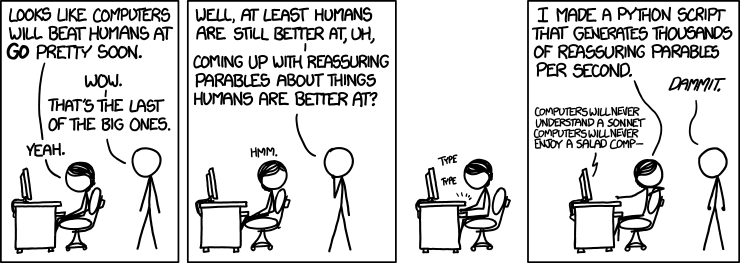
\includegraphics[width=0.7\textwidth]{reassuring}
\end{center}

\paragraph{Objectives}

Students completing this course will have an in-depth understanding of
three core areas of AI and the connections among them, and with such
other key AI areas as machine learning, robotics, natural language
processing and multi-agent systems. They should be able to:

\begin{itemize}
\item choose the appropriate representation for an AI problem or
  domain model, and construct domain models in that representation
\item choose the appropriate algorithm for reasoning within an AI
  problem domain
\item implement and debug core AI algorithms in a clean and structured
  manner
\item design and analyze the performance of an AI system
  or component
\item describe AI algorithms and representations and explain their
  performance, in writing and orally
\item critically read papers on AI systems
\end{itemize} 

\section{Preliminaries} 

\paragraph{Prerequisites}

CS 51 (experience with systems building and familiarity with
complexity). CS 121, CS 124, or CS 124 are recommend and may be taken
concurrently. No previous exposure to AI is assumed. Talk to the
instructor if you're concerned about your preparation.  Programming
assignments will use the language Python; an introduction to the
language will be given in the first week.

\paragraph{Textbook}

The main textbook for the course is \textbf{Artificial Intelligence: A
  Modern Approach} (3rd edition) by Stuart Russell and Peter Norvig,
a.k.a AIMA(3e). It is available in the COOP. In addition to the
textbook, we will also read several research papers during the
term. Finally, the course staff is always happy to recommend
additional readings or other sources of information if you would like
to explore a topic from the course in more depth.

\paragraph{Laptop Policy}

For the sake of cutting down on distraction and maintaining an
academic atmosphere, phones and laptops will in general not be
permitted during lecture. As we understand that some students prefer
laptops for note-taking, we ask that you contact the course staff at
the beginning of the semester if you require your laptop during
class. We will also ask that students using laptops sit in a designated
section so as not to distract other colleagues.

\paragraph{Support resources}

We will be using the Piazza for questions. Unless your question would
reveal confidential information or give away answers to homework
questions, please post there. We also encourage you to answer each
others questions.

\paragraph{Office hours} 
The staff office hours will be posted on the
website. You are welcome to come with specific questions about the
material, to discuss final project ideas, or just to chat about things
you find interesting and want to explore further.

\paragraph{Email} Staff emails are posted on the website. To avoid
duplication of questions and keep the email load manageable, please
use the forums if your question may be of interest to other students,
and only use email for personal questions.

\section{Provisional Schedule}

This weekly schedule is provisional. It may be adjusted based on the observed pace of the course:
\vspace {0.25cm}

 \begin{center}
\begin{tabular}{llll}
\toprule
Date &Topic &Readings &Assignment \\
\midrule
 Sept. 3 & Artificial Intelligence  & AIMA 1 &HW 0 \\
 Sept. 8 &Search 1: Formalism & AIMA 3.1-3.4  &HW 1 \\
 Sept. 10 & Search 2: Uninformed Search  & AIMA 3.5,3.6 & \\
 Sept. 15 & Search 3: A* and Heuristics & &HW 2 \\
 Sept. 17 &Adversarial Search &AIMA 5 & \\
 Sept. 22 & Paper Discussion 1  & & \\
 Sept. 25 &Constraint Satisfaction &AIMA 6.1-6.3 & \\ 
 Sept. 29 &CSP, Local Search, and Optimization &AIMA 4.1, 6.4 & HW 3 \\ 
 Oct. 1 & Propositional Logic and Satisfiability &AIMA 7 &  \\
 Oct. 6 & Propositional Logic and Resolution &  & \\ 
 Oct. 8 & Planning & AIMA 10 & \\ 
 Oct. 13 & Paper Discussion 2 & & \\
 Oct. 15 & Applications in NLP/Vision/Robotics 1 & & \\
 Oct. 20 & Midterm 1 (Search, CSP, Logic) & & \\
 Oct. 22 & Markov Decision Processes 1 &AIMA 17.1-17.3 & \\
 Oct. 27 & Markov Decision Processes 2  & & \\
 Oct. 29 & Baysian Networks: Representation &AIMA 14 &HW 5 \\
 Nov. 3 & Baysian Networks: Independence & & \\
 Nov. 5 & Baysian Networks: Inference & & \\
 Nov. 10 & Markov Models &AIMA 15.1-15.3 & \\
 Nov. 12 & Hidden Markov Models & & \\
 Nov. 17 & Applications in NLP/Vision/Robotics 2  & & \\
 Nov. 19 & Midterm 2 (MDPs, Bayes nets, HMMs)  & & \\
 Nov. 24 & Guest Lecture - Machine Learning && Project Update \\
 Dec. 1 & Paper Discussion 3  & & \\
 Dec. 3 & Final Project Presentations 1  & & \\
 Dec. 8 & Final Project Presentations 2 & & \\
 Dec. 10 & Final Project Due  & &\\
\bottomrule
\end{tabular}
 \end{center}

\vspace {0.25cm}
\section{Course Requirements}

The course has several components:

\begin{itemize}
\item Six assignments; each will have a computational part and written part (50\%)
\item Two in-class exams (October 20 and November 19) (25\%)
\item A final project (done in pairs) (20\%)
\item Paper reviews and discussion (5\%)
\end{itemize}


\noindent Final grades take into account each component. You must achieve a passing grade in all components to pass this course. To receive an A you must have high performance is all categories.

\paragraph{Assignments}

The 6 assignments (HW 0 - HW 5) will be published on the course
webpage. Also see the collaboration policy below.

Most assignments have two components: computational and written. The
computational part can be done in pairs or individually and will
require programming and experimentation. The written part will be
submitted individually and will include analysis of the results.
Computational assignments will ask you to develop implementations of
algorithms for search, game-solving, constraint satisfaction,
knowledge representation and reasoning, and planning, to apply them to
different real-world problems, and to analyze the performance. We
expect that all code will run, be well-written and be commented
appropriately; the course staff is always happy to help explain style
and conventions.  The written components ask you questions about the
concepts and methods that you have learned and to reflect on the
performance of your implementations.

\paragraph{Late days} As students tend to be over-committed, each
student is allotted \textbf{five} late days which may be applied to
any of the assignments.  You must \textbf{email} the TF for a late day
to apply. A late day extends the due date by 24 hours. No more than
two late days may be used on any one assignment. In cases of medical
or other emergencies which interfere with your work, have your senior
tutor contact the instructor. 

\paragraph{Grading} Assignments will be due at \textbf{5pm} on the day
scheduled. If you have used up your 5 late days, you will be penalized
25\% per day, up to two days max, with no credit after two days. We
will only give extensions for emergencies, and you will need a note
from either a doctor or your Resident Dean. Any grading disputes,
aside from arithmetic errors, will go to the head TF, and the work in
question will be fully regraded; the grade may go up or down as a
result. Computational components will be graded based on correctness,
performance and documentation.  Written components will be graded
based on correctness, depth of analysis, and clarity.

\paragraph{Readings}

Each class meeting is preceded by a reading assignment. It is
important to keep on top of the reading, which will be assumed during
the lecture and discussion in class. You should set aside 2 hours to
compete each reading. We do not expect you to fully understand
everything before coming to class, but the goal is to prepare for
class, familiarize yourself with new terminology and definitions, and
to determine which part of the subject you want to hear more about.
We encourage you to bring questions to class about material that is
confusing.  Other students might share your confusion.

\paragraph{Participation and Discussion}

We will have three paper discussion sessions. You are
expected to read the paper before class and should post a question in
the forum that is designated for discussion of that paper. The post
should contain a thought provoking question about the assigned paper
and is due no later than midnight of the night before the class
meeting.

We will offer two sources of additional credit in the class for
participation. First for students who go out of their way to provide
support in the Piazza forums, and second for students who
find bugs or errata in the course lecture notes or homeworks. For the
second, please email the professor with the subject \texttt{CS182
  Errata} in the subject line.


\paragraph{In-class Exams}

In addition to homework assignments, there are two in-class exams
(closed book, no notes), one covering the first half of the course
material and the second covering the second half of the course
material. See the schedule for dates and topics covered. The sections
preceding the class days will be exam reviews.

\paragraph{Final Project}

During the second half of the course students will design and carry
out a final project, working in pairs. The final project is of your
choosing: it can describe a system you have built or discuss more
theoretical issues or even survey cutting edge work in an active area
of AI research. We will provide a list of potential topics and an
opportunity to get feedback before starting. Most people who have
taken the course consider this one of the most fun and rewarding parts
of the course, and we hope you'll have fun with it too. The final
presentation and paper (by the group) are due at the end of reading
period, and attendance at the final presentation sessions is
mandatory.

The project grade is based three aspects: 
\begin{enumerate}
\item project concepts and results 
\item presentation quality 
\item final paper quality 
\end{enumerate}

\paragraph{Collaboration Policy}

Each assignment will include a computational component and a written component.

HW 0 must be done individually. The computational component of assignments 1-5 can done and submitted in pairs. In pairs implies designing and writing the code together and submitting a single assignment and receiving the same grade. Note that we will treat pairs/non-pairs the same from a grading perspective.  We expect you and your partner to design and implement the solutions together. You may also consult with your classmates in other groups as you work on the problem, but you should not talk in terms of pseudocode or real code, and you should not share answers. In addition, you must cite any books, articles, websites, lectures, etc. that have helped you with your work. Similarly, you must list the names of students from other groups with whom your group has collaborated. If you are doing the computational assignment individually, then the same rules apply for collaboration as for the written assignments: talking is ok, sharing code is not.

The written component of all assignments must be done individually, and each person must submit her/his own written assignment. You are encouraged to consult with your classmates as you work on the problems for the written assignments. However, you should not share answers.  After discussions with your peers, make sure that you can work through the problem yourself and ensure that any answers you submit for evaluation are the result of your own efforts. In addition, you must cite any books, articles, websites, lectures, etc. that have helped you with your work. Similarly, you must list the names of students with who you have collaborated.  Note that understanding the concepts in the written assignments is important both for the computational components and the exams. Final projects must be done in pairs. You are encouraged to discuss your project ideas with your peers.

For any questions not covered in this document, email the course staff for clarification.



\end{document}